% Options for packages loaded elsewhere
\PassOptionsToPackage{unicode}{hyperref}
\PassOptionsToPackage{hyphens}{url}
\PassOptionsToPackage{dvipsnames,svgnames,x11names}{xcolor}
\documentclass[
  brazilian,
  11pt,
]{article}
\usepackage{xcolor}
\usepackage[margin=2.4cm]{geometry}
\usepackage{amsmath,amssymb}
\setcounter{secnumdepth}{-\maxdimen} % remove section numbering
\usepackage{iftex}
\ifPDFTeX
  \usepackage[T1]{fontenc}
  \usepackage[utf8]{inputenc}
  \usepackage{textcomp} % provide euro and other symbols
\else % if luatex or xetex
  \usepackage{unicode-math} % this also loads fontspec
  \defaultfontfeatures{Scale=MatchLowercase}
  \defaultfontfeatures[\rmfamily]{Ligatures=TeX,Scale=1}
\fi
\usepackage{lmodern}
\ifPDFTeX\else
  % xetex/luatex font selection
\fi
% Use upquote if available, for straight quotes in verbatim environments
\IfFileExists{upquote.sty}{\usepackage{upquote}}{}
\IfFileExists{microtype.sty}{% use microtype if available
  \usepackage[]{microtype}
  \UseMicrotypeSet[protrusion]{basicmath} % disable protrusion for tt fonts
}{}
\makeatletter
\@ifundefined{KOMAClassName}{% if non-KOMA class
  \IfFileExists{parskip.sty}{%
    \usepackage{parskip}
  }{% else
    \setlength{\parindent}{0pt}
    \setlength{\parskip}{6pt plus 2pt minus 1pt}}
}{% if KOMA class
  \KOMAoptions{parskip=half}}
\makeatother
\usepackage{color}
\usepackage{fancyvrb}
\newcommand{\VerbBar}{|}
\newcommand{\VERB}{\Verb[commandchars=\\\{\}]}
\DefineVerbatimEnvironment{Highlighting}{Verbatim}{commandchars=\\\{\}}
% Add ',fontsize=\small' for more characters per line
\usepackage{framed}
\definecolor{shadecolor}{RGB}{35,38,41}
\newenvironment{Shaded}{\begin{snugshade}}{\end{snugshade}}
\newcommand{\AlertTok}[1]{\textcolor[rgb]{0.58,0.85,0.30}{\textbf{\colorbox[rgb]{0.30,0.12,0.14}{#1}}}}
\newcommand{\AnnotationTok}[1]{\textcolor[rgb]{0.25,0.50,0.35}{#1}}
\newcommand{\AttributeTok}[1]{\textcolor[rgb]{0.16,0.50,0.73}{#1}}
\newcommand{\BaseNTok}[1]{\textcolor[rgb]{0.96,0.45,0.00}{#1}}
\newcommand{\BuiltInTok}[1]{\textcolor[rgb]{0.50,0.55,0.55}{#1}}
\newcommand{\CharTok}[1]{\textcolor[rgb]{0.24,0.68,0.91}{#1}}
\newcommand{\CommentTok}[1]{\textcolor[rgb]{0.48,0.49,0.49}{#1}}
\newcommand{\CommentVarTok}[1]{\textcolor[rgb]{0.50,0.55,0.55}{#1}}
\newcommand{\ConstantTok}[1]{\textcolor[rgb]{0.15,0.68,0.68}{\textbf{#1}}}
\newcommand{\ControlFlowTok}[1]{\textcolor[rgb]{0.99,0.74,0.29}{\textbf{#1}}}
\newcommand{\DataTypeTok}[1]{\textcolor[rgb]{0.16,0.50,0.73}{#1}}
\newcommand{\DecValTok}[1]{\textcolor[rgb]{0.96,0.45,0.00}{#1}}
\newcommand{\DocumentationTok}[1]{\textcolor[rgb]{0.64,0.20,0.25}{#1}}
\newcommand{\ErrorTok}[1]{\textcolor[rgb]{0.85,0.27,0.33}{\underline{#1}}}
\newcommand{\ExtensionTok}[1]{\textcolor[rgb]{0.00,0.60,1.00}{\textbf{#1}}}
\newcommand{\FloatTok}[1]{\textcolor[rgb]{0.96,0.45,0.00}{#1}}
\newcommand{\FunctionTok}[1]{\textcolor[rgb]{0.56,0.27,0.68}{#1}}
\newcommand{\ImportTok}[1]{\textcolor[rgb]{0.15,0.68,0.38}{#1}}
\newcommand{\InformationTok}[1]{\textcolor[rgb]{0.77,0.36,0.00}{#1}}
\newcommand{\KeywordTok}[1]{\textcolor[rgb]{0.81,0.81,0.76}{\textbf{#1}}}
\newcommand{\NormalTok}[1]{\textcolor[rgb]{0.81,0.81,0.76}{#1}}
\newcommand{\OperatorTok}[1]{\textcolor[rgb]{0.81,0.81,0.76}{#1}}
\newcommand{\OtherTok}[1]{\textcolor[rgb]{0.15,0.68,0.38}{#1}}
\newcommand{\PreprocessorTok}[1]{\textcolor[rgb]{0.15,0.68,0.38}{#1}}
\newcommand{\RegionMarkerTok}[1]{\textcolor[rgb]{0.16,0.50,0.73}{\colorbox[rgb]{0.08,0.19,0.26}{#1}}}
\newcommand{\SpecialCharTok}[1]{\textcolor[rgb]{0.24,0.68,0.91}{#1}}
\newcommand{\SpecialStringTok}[1]{\textcolor[rgb]{0.85,0.27,0.33}{#1}}
\newcommand{\StringTok}[1]{\textcolor[rgb]{0.96,0.31,0.31}{#1}}
\newcommand{\VariableTok}[1]{\textcolor[rgb]{0.15,0.68,0.68}{#1}}
\newcommand{\VerbatimStringTok}[1]{\textcolor[rgb]{0.85,0.27,0.33}{#1}}
\newcommand{\WarningTok}[1]{\textcolor[rgb]{0.85,0.27,0.33}{#1}}
\usepackage{graphicx}
\makeatletter
\newsavebox\pandoc@box
\newcommand*\pandocbounded[1]{% scales image to fit in text height/width
  \sbox\pandoc@box{#1}%
  \Gscale@div\@tempa{\textheight}{\dimexpr\ht\pandoc@box+\dp\pandoc@box\relax}%
  \Gscale@div\@tempb{\linewidth}{\wd\pandoc@box}%
  \ifdim\@tempb\p@<\@tempa\p@\let\@tempa\@tempb\fi% select the smaller of both
  \ifdim\@tempa\p@<\p@\scalebox{\@tempa}{\usebox\pandoc@box}%
  \else\usebox{\pandoc@box}%
  \fi%
}
% Set default figure placement to htbp
\def\fps@figure{htbp}
\makeatother
\ifLuaTeX
\usepackage[bidi=basic,shorthands=off]{babel}
\else
\usepackage[bidi=default,shorthands=off]{babel}
\fi
\ifLuaTeX
  \usepackage{selnolig} % disable illegal ligatures
\fi
\setlength{\emergencystretch}{3em} % prevent overfull lines
\providecommand{\tightlist}{%
  \setlength{\itemsep}{0pt}\setlength{\parskip}{0pt}}
% ==========================================================================
%  Cabecalho LaTeX do curso "Trabalhando com Texto em Python I"
%  Injetado pelo pandoc (-H) ao gerar o .tex de cada unidade.
% ==========================================================================
\usepackage[T1]{fontenc}
\usepackage{lmodern}
\usepackage[scaled=0.92]{helvet}
\renewcommand{\familydefault}{\sfdefault}
\usepackage{microtype}
\usepackage{amssymb}
\usepackage{newunicodechar}
\usepackage{xcolor}
\usepackage[most]{tcolorbox}
\tcbuselibrary{skins,breakable}
\usepackage{titlesec}
\usepackage{enumitem}
% quebra linhas longas nos blocos de codigo (evita vazar a margem)
\usepackage{fvextra}
\fvset{breaklines=true,breakanywhere=true,fontsize=\small}

% -------- paleta --------
\definecolor{accent}{HTML}{6C4CF1}
\definecolor{cyan}{HTML}{00B4D8}
\definecolor{subink}{HTML}{2B3242}
\definecolor{notec}{HTML}{3B82F6}
\definecolor{tipc}{HTML}{10B981}
\definecolor{warnc}{HTML}{F59E0B}

% -------- emojis / simbolos unicode que podem aparecer no texto --------
% simbolos com significado
\newunicodechar{✅}{{\color{tipc}\checkmark}}
\newunicodechar{✔}{{\color{tipc}\checkmark}}
\newunicodechar{☐}{$\square$}
\newunicodechar{κ}{\ensuremath{\kappa}}
\newunicodechar{≈}{\ensuremath{\approx}}
\newunicodechar{−}{\ensuremath{-}}
\newunicodechar{↓}{\ensuremath{\downarrow}}
\newunicodechar{→}{\ensuremath{\rightarrow}}
\newunicodechar{←}{\ensuremath{\leftarrow}}
\newunicodechar{↹}{\ensuremath{\hookrightarrow}}
\newunicodechar{°}{\textdegree}
\newunicodechar{·}{\textperiodcentered}
\newunicodechar{´}{'}
\newunicodechar{‑}{-}
% emojis decorativos -> removidos no PDF
\newunicodechar{💡}{}
\newunicodechar{🚀}{}
\newunicodechar{📝}{}
\newunicodechar{⚠}{}
\newunicodechar{🐍}{}
\newunicodechar{🎉}{}
\newunicodechar{🍕}{}
\newunicodechar{👍}{}
\newunicodechar{💋}{}
\newunicodechar{😚}{}
\newunicodechar{🚂}{}
\newunicodechar{❤}{}

% -------- caixas de callout (usadas pelo filtro callouts.lua) --------
\newtcolorbox{notebox}{enhanced,breakable,colback=notec!6,colframe=notec,
  boxrule=0pt,leftrule=4pt,arc=3pt,left=10pt,right=10pt,top=7pt,bottom=7pt,
  before skip=10pt,after skip=12pt}
\newtcolorbox{tipbox}{enhanced,breakable,colback=tipc!7,colframe=tipc,
  boxrule=0pt,leftrule=4pt,arc=3pt,left=10pt,right=10pt,top=7pt,bottom=7pt,
  before skip=10pt,after skip=12pt}
\newtcolorbox{warnbox}{enhanced,breakable,colback=warnc!8,colframe=warnc,
  boxrule=0pt,leftrule=4pt,arc=3pt,left=10pt,right=10pt,top=7pt,bottom=7pt,
  before skip=10pt,after skip=12pt}
\newtcolorbox{objbox}{enhanced,breakable,colback=accent!5,colframe=accent,
  boxrule=0pt,leftrule=4pt,arc=3pt,left=10pt,right=10pt,top=7pt,bottom=8pt,
  before skip=10pt,after skip=14pt}

% -------- titulos coloridos --------
\titleformat{\section}{\sffamily\Large\bfseries\color{accent}}{\thesection}{0.6em}{}
\titleformat{\subsection}{\sffamily\large\bfseries\color{subink}}{\thesubsection}{0.5em}{}
\titleformat{\subsubsection}{\sffamily\normalsize\bfseries\color{cyan}}{\thesubsubsection}{0.5em}{}
\titlespacing*{\section}{0pt}{2.2ex plus 1ex minus .2ex}{1.1ex}

% codigo inline colorido
\definecolor{inlink}{HTML}{5A34D6}
\let\oldtexttt\texttt
\renewcommand{\texttt}[1]{{\color{inlink}\oldtexttt{#1}}}
\usepackage{bookmark}
\IfFileExists{xurl.sty}{\usepackage{xurl}}{} % add URL line breaks if available
\urlstyle{same}
% fallback for those not using the hyperref driver hyperxmp:
\makeatletter
\@ifundefined{xmpquote}{\newcommand{\xmpquote}[1]{#1}}{}
\makeatother
\hypersetup{
  pdftitle={Processando textos com spaCy},
  pdfauthor={CiberExt 26-29 · FEELT38103 · Universidade Federal de Uberlândia},
  pdflang={pt-BR},
  colorlinks=true,
  linkcolor={accent},
  filecolor={Maroon},
  citecolor={Blue},
  urlcolor={cyan},
  pdfcreator={LaTeX via pandoc}}

\title{Processando textos com spaCy}
\usepackage{etoolbox}
\makeatletter
\providecommand{\subtitle}[1]{% add subtitle to \maketitle
  \apptocmd{\@title}{\par {\large #1 \par}}{}{}
}
\makeatother
\subtitle{Trabalhando com Texto em Python I · Unidade 2}
\author{CiberExt 26-29 · FEELT38103 · Universidade Federal de
Uberlândia}
\date{2026}

\begin{document}
\maketitle

{
\setcounter{tocdepth}{2}
\tableofcontents
}
\subsubsection{Objetivos de
aprendizagem}\label{objetivos-de-aprendizagem}

Ao final desta unidade, você deverá:

\begin{itemize}
\tightlist
\item
  conhecer alguns dos \textbf{conceitos e tarefas fundamentais} do
  processamento de linguagem natural (PLN);
\item
  saber \textbf{realizar tarefas simples} de PLN usando a biblioteca
  \textbf{spaCy}.
\end{itemize}

\begin{center}\rule{0.5\linewidth}{0.5pt}\end{center}

\subsection{1. Primeiros passos}\label{primeiros-passos}

Para começar, importamos o \textbf{spaCy}, uma das muitas bibliotecas
disponíveis para processamento de linguagem natural em Python.

\begin{Shaded}
\begin{Highlighting}[]
\CommentTok{\# Importa a biblioteca spaCy}
\ImportTok{import}\NormalTok{ spacy}
\end{Highlighting}
\end{Shaded}

\begin{tipbox}

\textbf{Dica prática:} a primeira importação do spaCy pode demorar
alguns segundos, porque a biblioteca carrega dependências pesadas (redes
neurais, tokenizadores etc.). Isso é normal.

\end{tipbox}

Para realizar tarefas de processamento de linguagem natural em um idioma
específico, precisamos carregar um \textbf{modelo de linguagem} treinado
para executar essas tarefas naquele idioma.

O spaCy oferece suporte a muitos idiomas, mas disponibiliza
\textbf{modelos pré‑treinados} apenas para um subconjunto deles. Esses
modelos vêm em tamanhos e ``sabores'' diferentes --- exploraremos essas
diferenças mais adiante no curso. Para nos familiarizarmos com as
tarefas básicas de PLN, começaremos com um modelo pequeno para o
\textbf{inglês}.

Os modelos de linguagem são carregados com a função \texttt{load()} do
spaCy, que recebe o \textbf{nome do modelo} como entrada:

\begin{Shaded}
\begin{Highlighting}[]
\CommentTok{\# Carrega o modelo pequeno de lingua inglesa e o atribui a variavel \textquotesingle{}nlp\textquotesingle{}}
\NormalTok{nlp }\OperatorTok{=}\NormalTok{ spacy.load(}\StringTok{\textquotesingle{}en\_core\_web\_sm\textquotesingle{}}\NormalTok{)}

\CommentTok{\# Chama a variavel para examinar o objeto}
\NormalTok{nlp}
\end{Highlighting}
\end{Shaded}

Chamar a variável \texttt{nlp} retorna um objeto \texttt{Language} do
spaCy, que contém o modelo de linguagem para o inglês. Em essência, o
objeto \texttt{Language} do spaCy é um \textbf{pipeline} (uma sequência
de etapas de processamento) que usa o modelo de linguagem para executar
diversas tarefas de PLN --- tarefas que veremos a seguir.

\subsubsection{1.1 O que é um modelo de
linguagem?}\label{o-que-uxe9-um-modelo-de-linguagem}

A maioria dos modelos de linguagem modernos é baseada em
\textbf{estatística}, e não em regras definidas manualmente por humanos.
Modelos de linguagem estatísticos se apoiam em \textbf{probabilidades},
respondendo perguntas como:

\begin{itemize}
\tightlist
\item
  Qual a probabilidade de uma determinada frase ocorrer em um idioma?
\item
  Qual a probabilidade de uma determinada palavra ocorrer em uma
  sequência de palavras?
\end{itemize}

Considere as frases a seguir, extraídas dos artigos de jornal usados na
unidade anterior:

\begin{quote}
\emph{``From financial exchanges in \textbf{OCULTO} Manhattan to
cloakrooms in Washington and homeless shelters in California, unfamiliar
rituals were the order of the day.''}

\emph{``Security precautions were being taken around the \textbf{OCULTO}
as the deadline for Iraq to withdraw from Kuwait neared.''}
\end{quote}

Você provavelmente consegue \textbf{arriscar um bom palpite} sobre as
palavras ocultas, com base no seu conhecimento da língua inglesa e do
mundo em geral (no primeiro caso, algo como \emph{``lower''}; no
segundo, \emph{``country''}).

Da mesma forma, construir um modelo de linguagem estatístico envolve
observar a ocorrência de palavras em \textbf{grandes corpora} e calcular
suas probabilidades de ocorrência em um determinado contexto. O modelo é
então treinado fazendo previsões e ajustando‑se com base nos erros
cometidos durante essas previsões.

\subsubsection{1.2 Como os modelos de linguagem são
treinados?}\label{como-os-modelos-de-linguagem-suxe3o-treinados}

O modelo pequeno para o inglês, por exemplo, é treinado em um corpus
chamado \textbf{OntoNotes 5.0}, que reúne textos de gêneros variados ---
notícias de agências de imprensa, notícias de telejornal, conversas
telefônicas e transmitidas, e blogs. Isso permite que o corpus cubra a
variação linguística tanto da língua \textbf{escrita} quanto
\textbf{falada} em inglês.

O corpus OntoNotes 5.0 é composto por mais do que texto puro: suas
anotações incluem \textbf{classes gramaticais} (\emph{part‑of‑speech
tags}), \textbf{dependências sintáticas} e \textbf{correferências} entre
palavras. Isso permite modelar não apenas a ocorrência de palavras ou
sequências de palavras, mas também suas \textbf{características
gramaticais}.

\begin{center}\rule{0.5\linewidth}{0.5pt}\end{center}

\subsection{2. Realizando tarefas básicas de PLN com
spaCy}\label{realizando-tarefas-buxe1sicas-de-pln-com-spacy}

Para processar um texto usando o objeto \texttt{Language} que contém o
modelo de linguagem para o inglês, basta \textbf{chamar} o objeto
\texttt{nlp} sobre algum texto.

Vamos definir uma frase de teste simples --- um objeto \emph{string} do
Python, guardado na variável \texttt{text}:

\begin{Shaded}
\begin{Highlighting}[]
\CommentTok{\# Atribui uma frase de exemplo a variavel \textquotesingle{}text\textquotesingle{}}
\NormalTok{text }\OperatorTok{=} \StringTok{"The Federal Bureau of Investigation has been ordered to track down as many as 3,000 Iraqis in this country whose visas have expired, the Justice Department said yesterday."}

\CommentTok{\# Chama a variavel para examinar o resultado}
\NormalTok{text}
\end{Highlighting}
\end{Shaded}

Passar a variável \texttt{text} para o objeto \texttt{Language}
\texttt{nlp} retorna um objeto \texttt{Doc} do spaCy (abreviação de
\emph{document}, ``documento''). Em processamento de linguagem natural,
trechos maiores de texto costumam ser chamados de ``documentos'', ainda
que, neste caso, nosso documento consista em uma única frase.

Esse objeto contém tanto o texto de entrada (\texttt{text}) quanto os
\textbf{resultados} do processamento de linguagem natural feito pelo
spaCy.

\begin{Shaded}
\begin{Highlighting}[]
\CommentTok{\# Alimenta a string em \textquotesingle{}text\textquotesingle{} ao objeto Language em \textquotesingle{}nlp\textquotesingle{}}
\CommentTok{\# Guarda o resultado na variavel \textquotesingle{}doc\textquotesingle{}}
\NormalTok{doc }\OperatorTok{=}\NormalTok{ nlp(text)}
\end{Highlighting}
\end{Shaded}

O objeto \texttt{Doc} agora está guardado na variável \texttt{doc}:

\begin{Shaded}
\begin{Highlighting}[]
\CommentTok{\# Chama a variavel para examinar o objeto}
\NormalTok{doc}
\end{Highlighting}
\end{Shaded}

Embora a saída se pareça com uma \emph{string} comum do Python, o objeto
\texttt{Doc} contém uma \textbf{riqueza de informações} sobre a
estrutura linguística do texto, geradas pelo spaCy ao processar a frase
através do seu \emph{pipeline} de PLN. Vamos agora examinar, uma a uma,
as tarefas realizadas ``nos bastidores''.

\begin{figure}
\centering
\pandocbounded{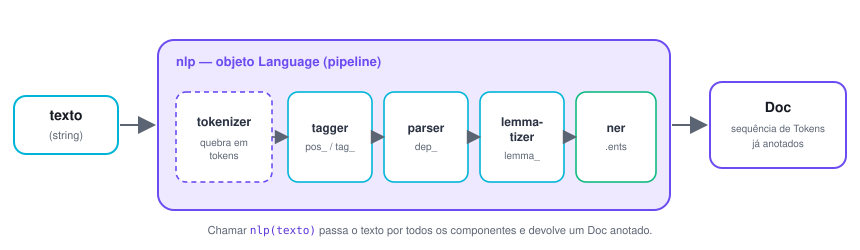
\includegraphics[keepaspectratio,alt={O pipeline de PLN do spaCy: chamar nlp(texto) passa o texto por vários componentes (tokenizer, tagger, parser, lematizador, NER) e devolve um objeto Doc já anotado.}]{img/pipeline-spacy.pdf}}
\caption{O \emph{pipeline} de PLN do spaCy: chamar
\protect\texttt{nlp(texto)} passa o texto por vários componentes
(tokenizer, tagger, parser, lematizador, NER) e devolve um objeto
\protect\texttt{Doc} já anotado.}
\end{figure}

\subsubsection{2.1 Tokenização}\label{tokenizauxe7uxe3o}

A primeira tarefa realizada é conhecida como \textbf{tokenização}: ela
quebra o texto em unidades analíticas que serão processadas
posteriormente.

Na maioria dos casos, um \textbf{token} corresponde a uma palavra
separada por espaço em branco, mas sinais de pontuação também são
considerados tokens independentes. Como os computadores tratam palavras
como sequências de caracteres, atribuir aos sinais de pontuação seus
próprios tokens evita que a pontuação final ``grude'' nas palavras que a
precedem.

Um objeto \texttt{Doc} do spaCy é composto por uma sequência de objetos
\texttt{Token}, que armazenam os resultados das diversas tarefas de PLN.
Vamos imprimir cada objeto \texttt{Token} guardado em \texttt{doc}:

\begin{Shaded}
\begin{Highlighting}[]
\CommentTok{\# Percorre os itens no objeto Doc, usando a variavel \textquotesingle{}token\textquotesingle{} para se referir aos itens da lista}
\ControlFlowTok{for}\NormalTok{ token }\KeywordTok{in}\NormalTok{ doc:}

    \CommentTok{\# Imprime cada token}
    \BuiltInTok{print}\NormalTok{(token)}
\end{Highlighting}
\end{Shaded}

A saída mostra um \texttt{Token} por linha. Como esperado, sinais de
pontuação como \texttt{.} e \texttt{,} constituem seus próprios
\texttt{Token}s.

\subsubsection{\texorpdfstring{2.2 Anotação morfossintática
(\emph{part‑of‑speech
tagging})}{2.2 Anotação morfossintática (part‑of‑speech tagging)}}\label{anotauxe7uxe3o-morfossintuxe1tica-partofspeech-tagging}

A \textbf{anotação morfossintática} (\emph{POS tagging}) é a tarefa de
determinar a \textbf{classe gramatical} de um token. Isso é crucial para
desambiguação, já que classes gramaticais diferentes podem ter formas
idênticas.

Considere o exemplo em inglês: \emph{``The sailor \textbf{dogs} the
hatch.''} (algo como ``O marinheiro tranca a escotilha''). O presente do
verbo \emph{to dog} (prender/trancar algo com algo) é exatamente igual
ao plural do substantivo \emph{dog} (cachorro): \texttt{dogs}. Para
identificar a classe correta, é preciso examinar o \textbf{contexto} em
que a palavra aparece.

O spaCy fornece dois tipos de anotação morfossintática, uma
\textbf{genérica} (\emph{coarse}) e uma \textbf{detalhada}
(\emph{fine‑grained}), guardadas respectivamente nos atributos
\texttt{pos\_} e \texttt{tag\_}. Acessamos os atributos de um objeto
Python inserindo o atributo após o objeto, separados por um ponto final
--- por exemplo, \texttt{token.pos\_}.

\begin{Shaded}
\begin{Highlighting}[]
\CommentTok{\# Percorre os itens no objeto Doc, usando a variavel \textquotesingle{}token\textquotesingle{} para se referir aos itens da lista}
\ControlFlowTok{for}\NormalTok{ token }\KeywordTok{in}\NormalTok{ doc:}

    \CommentTok{\# Imprime o token e as anotacoes morfossintaticas genericas e detalhadas}
    \BuiltInTok{print}\NormalTok{(token, token.pos\_, token.tag\_)}
\end{Highlighting}
\end{Shaded}

As anotações genéricas disponíveis em \texttt{pos\_} são baseadas no
conjunto de rótulos do projeto \textbf{Universal Dependencies}. Já as
anotações detalhadas em \texttt{tag\_} são baseadas no corpus OntoNotes
5.0 apresentado acima. Diferentemente das anotações genéricas, as
detalhadas também codificam informação gramatical adicional --- as
anotações de verbos, por exemplo, se distinguem por \textbf{aspecto} e
\textbf{tempo verbal}.

\subsubsection{2.3 Análise morfológica}\label{anuxe1lise-morfoluxf3gica}

\textbf{Morfemas} são as menores unidades gramaticais que carregam
significado. Reconhecem‑se geralmente dois tipos: \textbf{morfemas
livres}, que consistem em palavras capazes de existir sozinhas, e
\textbf{morfemas presos}, que flexionam outros morfemas. No inglês,
morfemas presos incluem sufixos como \texttt{-s}, usado para indicar o
plural de um substantivo.

Em outras palavras, os morfemas moldam a forma externa de uma palavra, e
essas formas estão associadas a funções gramaticais específicas.

O spaCy realiza a análise morfológica automaticamente, guardando o
resultado no atributo \texttt{morph} de um objeto \texttt{Token}:

\begin{Shaded}
\begin{Highlighting}[]
\CommentTok{\# Percorre os itens no objeto Doc, usando a variavel \textquotesingle{}token\textquotesingle{} para se referir aos itens da lista}
\ControlFlowTok{for}\NormalTok{ token }\KeywordTok{in}\NormalTok{ doc:}

    \CommentTok{\# Imprime o token e o resultado da analise morfologica}
    \BuiltInTok{print}\NormalTok{(token, token.morph)}
\end{Highlighting}
\end{Shaded}

Como mostra a saída, \textbf{nem todos os tokens} têm informação
morfológica --- alguns consistem em morfemas livres, sem flexão. Para
recuperar informação morfológica de um \texttt{Token}, usamos o método
\texttt{get()} do atributo \texttt{morph}. Podemos usar colchetes
\texttt{{[}{]}} para acessar itens no objeto \texttt{Doc}. A linha a
seguir recupera a informação morfológica de \textbf{aspecto} para o 23º
token do \texttt{Doc} (índice 22):

\begin{Shaded}
\begin{Highlighting}[]
\CommentTok{\# Recupera informacao morfologica sobre aspecto para o Token no indice 22 do objeto Doc}
\NormalTok{doc[}\DecValTok{22}\NormalTok{].morph.get(}\StringTok{\textquotesingle{}Aspect\textquotesingle{}}\NormalTok{)}
\end{Highlighting}
\end{Shaded}

Isso retorna uma lista com um único item, a \emph{string} \texttt{Perf},
que se refere ao \textbf{aspecto perfectivo}.

O que acontece se tentarmos recuperar uma característica morfológica que
o token \textbf{não possui}? Vamos tentar recuperar a informação de
aspecto para o 22º token (índice 21):

\begin{Shaded}
\begin{Highlighting}[]
\CommentTok{\# Recupera informacao morfologica sobre aspecto para o Token no indice 21 do objeto Doc}
\NormalTok{doc[}\DecValTok{21}\NormalTok{].morph.get(}\StringTok{\textquotesingle{}Aspect\textquotesingle{}}\NormalTok{)}
\end{Highlighting}
\end{Shaded}

Isso retorna uma \textbf{lista vazia}, indicada pelos colchetes
\texttt{{[}\ {]}} sem nada entre eles.

Para recuperar \textbf{toda} a informação morfológica disponível para um
dado \texttt{Token}, a melhor solução é usar o método
\texttt{to\_dict()} do atributo \texttt{morph}. Isso retorna um
\textbf{dicionário}, uma estrutura de dados do Python composta por pares
de chave e valor:

\begin{Shaded}
\begin{Highlighting}[]
\CommentTok{\# Recupera informacao morfologica para o Token no indice 21 do objeto Doc}
\CommentTok{\# Usa o metodo to\_dict() para converter o resultado em um dicionario}
\NormalTok{doc[}\DecValTok{21}\NormalTok{].morph.to\_dict()}
\end{Highlighting}
\end{Shaded}

Um dicionário Python é delimitado por chaves \texttt{\{\ \}}. Cada par
chave/valor é separado por dois‑pontos \texttt{:}. Nesse caso, tanto as
chaves quanto os valores são objetos \emph{string}. O valor guardado em
uma chave pode ser acessado colocando o nome da chave entre colchetes
\texttt{{[}\ {]}} logo após o nome do dicionário:

\begin{Shaded}
\begin{Highlighting}[]
\CommentTok{\# Atribui a informacao morfologica ao dicionario \textquotesingle{}morph\_dict\textquotesingle{}}
\NormalTok{morph\_dict }\OperatorTok{=}\NormalTok{ doc[}\DecValTok{21}\NormalTok{].morph.to\_dict()}

\CommentTok{\# Recupera o valor correspondente a chave \textquotesingle{}Mood\textquotesingle{}}
\NormalTok{morph\_dict[}\StringTok{\textquotesingle{}Mood\textquotesingle{}}\NormalTok{]}
\end{Highlighting}
\end{Shaded}

Dicionários são uma estrutura de dados poderosa em Python, que usaremos
com frequência para guardar informações.

\subsubsection{\texorpdfstring{2.4 Análise sintática (\emph{parsing} de
dependências)}{2.4 Análise sintática (parsing de dependências)}}\label{anuxe1lise-sintuxe1tica-parsing-de-dependuxeancias}

A \textbf{análise sintática} (ou \emph{parsing} de dependências) é a
tarefa de definir as \textbf{dependências sintáticas} entre tokens.
Essas dependências ficam disponíveis no atributo \texttt{dep\_} de um
objeto \texttt{Token}:

\begin{Shaded}
\begin{Highlighting}[]
\CommentTok{\# Percorre os itens no objeto Doc, usando a variavel \textquotesingle{}token\textquotesingle{} para se referir aos itens da lista}
\ControlFlowTok{for}\NormalTok{ token }\KeywordTok{in}\NormalTok{ doc:}

    \CommentTok{\# Imprime o token e sua etiqueta de dependencia}
    \BuiltInTok{print}\NormalTok{(token, token.dep\_)}
\end{Highlighting}
\end{Shaded}

Diferentemente das anotações morfossintáticas, associadas a um único
\texttt{Token}, as etiquetas de dependência indicam uma \textbf{relação}
entre dois tokens. Para entender melhor essas relações sintáticas, vamos
usar alguns atributos adicionais de cada \texttt{Token}:

\begin{itemize}
\tightlist
\item
  \texttt{i}: a posição do token no \texttt{Doc};
\item
  \texttt{token}: o próprio token;
\item
  \texttt{dep\_}: a etiqueta da relação sintática;
\item
  \texttt{head} e \texttt{i}: o token que \textbf{governa} o token
  atual, e o índice desse token‑governante.
\end{itemize}

Isso ilustra como os atributos do Python podem ser combinados de forma
flexível: o atributo \texttt{head} aponta para outro \texttt{Token}, que
por sua vez tem o atributo \texttt{i} com seu próprio índice no
\texttt{Doc}. Podemos combinar os dois atributos e acessar essa
informação com \texttt{.head.i}:

\begin{Shaded}
\begin{Highlighting}[]
\CommentTok{\# Percorre os itens no objeto Doc, usando a variavel \textquotesingle{}token\textquotesingle{} para se referir aos itens da lista}
\ControlFlowTok{for}\NormalTok{ token }\KeywordTok{in}\NormalTok{ doc:}

    \CommentTok{\# Imprime o indice do token atual, o token, a dependencia, o governante e seu indice}
    \BuiltInTok{print}\NormalTok{(token.i, token, token.dep\_, token.head.i, token.head)}
\end{Highlighting}
\end{Shaded}

Embora a saída acima ajude a esclarecer as dependências sintáticas entre
os tokens, elas costumam ser \textbf{muito mais fáceis de perceber} por
meio de diagramas. O spaCy oferece uma ferramenta de visualização
chamada \textbf{displaCy}, importável com o comando:

\begin{Shaded}
\begin{Highlighting}[]
\ImportTok{from}\NormalTok{ spacy }\ImportTok{import}\NormalTok{ displacy}
\end{Highlighting}
\end{Shaded}

O módulo \texttt{displacy} tem uma função chamada \texttt{render()}, que
recebe um objeto \texttt{Doc} como entrada. Para desenhar uma árvore de
dependências, passamos o \texttt{Doc} \texttt{doc} à função
\texttt{render()} com dois argumentos:

\begin{itemize}
\tightlist
\item
  \texttt{style}: o valor
  \texttt{\textquotesingle{}dep\textquotesingle{}} instrui o displaCy a
  desenhar uma visualização de dependências sintáticas;
\item
  \texttt{options}: recebe um dicionário Python como entrada. Passamos
  um dicionário com a chave \texttt{compact} e o valor booleano
  \texttt{True} para instruir o displaCy a desenhar uma árvore compacta.
\end{itemize}

\begin{Shaded}
\begin{Highlighting}[]
\NormalTok{displacy.render(doc, style}\OperatorTok{=}\StringTok{\textquotesingle{}dep\textquotesingle{}}\NormalTok{, options}\OperatorTok{=}\NormalTok{\{}\StringTok{\textquotesingle{}compact\textquotesingle{}}\NormalTok{: }\VariableTok{True}\NormalTok{\})}
\end{Highlighting}
\end{Shaded}

As dependências sintáticas são visualizadas por meio de \textbf{linhas}
que partem do token‑governante em direção ao token governado por ele. As
etiquetas de dependência são baseadas no projeto \textbf{Universal
Dependencies}, um arcabouço para descrever características morfológicas
e sintáticas entre diferentes idiomas.

Se você não souber o significado de uma etiqueta específica, o spaCy
oferece uma função para explicá‑las, \texttt{explain()}, que recebe a
etiqueta como entrada (atenção: as etiquetas diferenciam maiúsculas de
minúsculas):

\begin{Shaded}
\begin{Highlighting}[]
\NormalTok{spacy.explain(}\StringTok{\textquotesingle{}pobj\textquotesingle{}}\NormalTok{)}
\end{Highlighting}
\end{Shaded}

Por fim, se você está se perguntando sobre os sublinhados \texttt{\_}
nos nomes dos atributos: o spaCy codifica todas as \emph{strings}
mapeando‑as para \textbf{valores de hash} (uma representação numérica)
por eficiência computacional. Vamos imprimir o primeiro token do
\texttt{Doc} (\texttt{doc{[}0{]}}) e suas dependências para examinar
como isso funciona:

\begin{Shaded}
\begin{Highlighting}[]
\BuiltInTok{print}\NormalTok{(doc[}\DecValTok{0}\NormalTok{], doc[}\DecValTok{0}\NormalTok{].dep, doc[}\DecValTok{0}\NormalTok{].dep\_)}
\end{Highlighting}
\end{Shaded}

Como se vê, o valor de hash \texttt{415} está reservado para a etiqueta
correspondente a um determinante (\texttt{det}).

\begin{warnbox}

\textbf{Atenção:} se você quiser uma saída legível para humanos na
análise de dependências e o spaCy devolver sequências de números,
provavelmente você esqueceu de adicionar o sublinhado ao nome do
atributo (por exemplo, usou \texttt{dep} em vez de \texttt{dep\_}).

\end{warnbox}

\subsubsection{2.5 Segmentação de
sentenças}\label{segmentauxe7uxe3o-de-sentenuxe7as}

O spaCy também segmenta objetos \texttt{Doc} em \textbf{sentenças} ---
tarefa conhecida como \textbf{segmentação de sentenças}. Essa
segmentação impõe estrutura adicional a textos maiores: ao determinar os
limites de uma sentença, podemos restringir tarefas como a análise de
dependências a sentenças individuais.

O spaCy disponibiliza o resultado da segmentação de sentenças no
atributo \texttt{sents} de um objeto \texttt{Doc}. Vamos percorrer as
sentenças contidas em \texttt{doc} e contá‑las usando a função
\texttt{enumerate()} do Python, que retorna uma contagem crescente a
cada item do laço:

\begin{Shaded}
\begin{Highlighting}[]
\CommentTok{\# Percorre as sentencas no objeto Doc e as conta usando enumerate()}
\ControlFlowTok{for}\NormalTok{ number, sent }\KeywordTok{in} \BuiltInTok{enumerate}\NormalTok{(doc.sents):}

    \CommentTok{\# Imprime o numero e a sentenca}
    \BuiltInTok{print}\NormalTok{(number, sent)}
\end{Highlighting}
\end{Shaded}

Isso retorna apenas \textbf{uma sentença}, mas o objeto \texttt{Doc}
poderia facilmente conter um texto mais longo com múltiplas sentenças,
como uma reportagem inteira.

\subsubsection{2.6 Lematização}\label{lematizauxe7uxe3o}

Um \textbf{lema} é a forma base de uma palavra. Tenha em mente que, a
menos que instruído explicitamente, o computador não sabe distinguir
formas singular e plural de uma palavra --- ele as trata como tokens
distintos, porque suas formas diferem.

Se quisermos contar a \textbf{ocorrência de palavras}, por exemplo, é
necessário um processo chamado \textbf{lematização}, que agrupa as
diferentes formas de um mesmo token. Os lemas ficam disponíveis para
cada \texttt{Token} no atributo \texttt{lemma\_}:

\begin{Shaded}
\begin{Highlighting}[]
\CommentTok{\# Percorre os itens no objeto Doc, usando a variavel \textquotesingle{}token\textquotesingle{} para se referir aos itens da lista}
\ControlFlowTok{for}\NormalTok{ token }\KeywordTok{in}\NormalTok{ doc:}

    \CommentTok{\# Imprime o token e seu lema}
    \BuiltInTok{print}\NormalTok{(token, token.lemma\_)}
\end{Highlighting}
\end{Shaded}

\subsubsection{\texorpdfstring{2.7 Reconhecimento de entidades nomeadas
(\emph{named entity recognition},
NER)}{2.7 Reconhecimento de entidades nomeadas (named entity recognition, NER)}}\label{reconhecimento-de-entidades-nomeadas-named-entity-recognition-ner}

O \textbf{reconhecimento de entidades nomeadas} (NER) é a tarefa de
identificar e classificar entidades mencionadas em um texto. O spaCy
reconhece as entidades nomeadas anotadas no corpus OntoNotes 5 ---
pessoas, locais geográficos e produtos, entre outros exemplos.

Usamos o atributo \texttt{.ents} do objeto \texttt{Doc} para obter as
entidades nomeadas:

\begin{Shaded}
\begin{Highlighting}[]
\NormalTok{doc.ents}
\end{Highlighting}
\end{Shaded}

Isso retorna uma \textbf{tupla} com as entidades nomeadas. Cada item da
tupla é um objeto \texttt{Span} do spaCy --- objetos \texttt{Span} podem
conter \textbf{múltiplos} objetos \texttt{Token}, já que muitas
entidades nomeadas se estendem por mais de um token. As entidades
nomeadas e seus tipos ficam guardados nos atributos \texttt{.text} e
\texttt{.label\_} de cada \texttt{Span}. Vamos percorrer a tupla e
imprimir ambos os atributos:

\begin{Shaded}
\begin{Highlighting}[]
\CommentTok{\# Percorre as entidades nomeadas no objeto Doc}
\ControlFlowTok{for}\NormalTok{ ent }\KeywordTok{in}\NormalTok{ doc.ents:}

    \CommentTok{\# Imprime a entidade nomeada e sua etiqueta}
    \BuiltInTok{print}\NormalTok{(ent.text, ent.label\_)}
\end{Highlighting}
\end{Shaded}

Como se vê, a maioria das entidades nomeadas identificadas consiste em
\textbf{múltiplos tokens}, por isso são representadas como objetos
\texttt{Span}. Podemos confirmar isso acessando a primeira entidade
nomeada (índice \texttt{0}, já que o Python conta do zero) e passando o
objeto à função \texttt{type()}:

\begin{Shaded}
\begin{Highlighting}[]
\CommentTok{\# Verifica o tipo do objeto usado para armazenar entidades nomeadas}
\BuiltInTok{type}\NormalTok{(doc.ents[}\DecValTok{0}\NormalTok{])}
\end{Highlighting}
\end{Shaded}

Objetos \texttt{Span} do spaCy têm vários argumentos úteis. Mais
importante: os atributos \texttt{start} e \texttt{end} retornam os
\textbf{índices dos tokens} que determinam onde o \texttt{Span} começa e
termina no \texttt{Doc}. Vamos examinar isso com mais detalhe,
imprimindo os atributos \texttt{start} e \texttt{end} da primeira
entidade nomeada:

\begin{Shaded}
\begin{Highlighting}[]
\CommentTok{\# Imprime a entidade nomeada e os indices de seus tokens de inicio e fim}
\BuiltInTok{print}\NormalTok{(doc.ents[}\DecValTok{0}\NormalTok{], doc.ents[}\DecValTok{0}\NormalTok{].start, doc.ents[}\DecValTok{0}\NormalTok{].end)}
\end{Highlighting}
\end{Shaded}

A entidade nomeada começa no índice \texttt{0} e termina no índice
\texttt{5} do \texttt{Doc}. Se recuperarmos o sexto token do
\texttt{Doc} (índice \texttt{5}), veremos que ele corresponde ao token
\texttt{"has"}:

\begin{Shaded}
\begin{Highlighting}[]
\NormalTok{doc[}\DecValTok{5}\NormalTok{]}
\end{Highlighting}
\end{Shaded}

Isso mostra que o índice retornado por \texttt{end} \textbf{não}
corresponde ao último token do \texttt{Span} que contém a entidade
nomeada, mas sim ao índice do \textbf{primeiro token seguinte} ao
\texttt{Span}. Vamos examinar isso percorrendo o recorte (\emph{slice})
do \texttt{Doc} correspondente à primeira entidade nomeada:

\begin{Shaded}
\begin{Highlighting}[]
\CommentTok{\# Percorre um recorte do objeto Doc que cobre a primeira entidade nomeada}
\ControlFlowTok{for}\NormalTok{ token }\KeywordTok{in}\NormalTok{ doc[doc.ents[}\DecValTok{0}\NormalTok{].start: doc.ents[}\DecValTok{0}\NormalTok{].end]:}

    \CommentTok{\# Imprime o token e seu indice}
    \BuiltInTok{print}\NormalTok{(token, token.i)}
\end{Highlighting}
\end{Shaded}

Como se vê, o atributo \texttt{start} indica onde o \texttt{Span}
\textbf{começa}, enquanto \texttt{end} indica onde o \texttt{Span}
\textbf{terminou} (ou seja, o token logo após o seu fim).

Também podemos renderizar as entidades nomeadas com o displaCy, o mesmo
módulo usado acima para visualizar as dependências sintáticas. Note que,
desta vez, passamos a \emph{string}
\texttt{\textquotesingle{}ent\textquotesingle{}} ao argumento
\texttt{style} para indicar que queremos visualizar \textbf{entidades
nomeadas}:

\begin{Shaded}
\begin{Highlighting}[]
\NormalTok{displacy.render(doc, style}\OperatorTok{=}\StringTok{\textquotesingle{}ent\textquotesingle{}}\NormalTok{)}
\end{Highlighting}
\end{Shaded}

Se você não reconhecer uma etiqueta usada para uma entidade nomeada,
pode sempre pedir uma explicação ao spaCy:

\begin{Shaded}
\begin{Highlighting}[]
\NormalTok{spacy.explain(}\StringTok{\textquotesingle{}NORP\textquotesingle{}}\NormalTok{)}
\end{Highlighting}
\end{Shaded}

\begin{center}\rule{0.5\linewidth}{0.5pt}\end{center}

\subsection{Quiz}\label{quiz}

Marque a alternativa correta (a resposta certa está destacada com ✅).

\textbf{1. A tarefa que quebra o texto em unidades menores chama‑se:}

\begin{enumerate}
\def\labelenumi{\arabic{enumi}.}
\tightlist
\item
  Tokenização ✅
\item
  Lematização
\item
  Segmentação de sentenças
\end{enumerate}

\textbf{2. Qual atributo do token dá a classe gramatical genérica?}

\begin{enumerate}
\def\labelenumi{\arabic{enumi}.}
\tightlist
\item
  \texttt{pos\_} ✅
\item
  \texttt{tag\_}
\item
  \texttt{dep\_}
\end{enumerate}

\textbf{3. O lema de uma palavra é:}

\begin{enumerate}
\def\labelenumi{\arabic{enumi}.}
\tightlist
\item
  A forma base da palavra ✅
\item
  Sempre o plural
\item
  A raiz fonética
\end{enumerate}

\textbf{4. As entidades nomeadas de um \texttt{Doc} ficam em qual
atributo?}

\begin{enumerate}
\def\labelenumi{\arabic{enumi}.}
\tightlist
\item
  \texttt{.ents} ✅
\item
  \texttt{.sents}
\item
  \texttt{.noun\_chunks}
\end{enumerate}

\textbf{5. Por que muitos atributos têm uma versão terminada em
sublinhado (ex.: \texttt{dep\_})?}

\begin{enumerate}
\def\labelenumi{\arabic{enumi}.}
\tightlist
\item
  Ela dá o texto legível, em vez do código numérico (hash) ✅
\item
  Ela é mais rápida
\item
  Ela é obrigatória
\end{enumerate}

\textbf{6. Uma entidade nomeada com vários tokens é representada por um
objeto:}

\begin{enumerate}
\def\labelenumi{\arabic{enumi}.}
\tightlist
\item
  \texttt{Span} ✅
\item
  \texttt{Token}
\item
  \texttt{Doc}
\end{enumerate}

\subsection{Resumo da unidade}\label{resumo-da-unidade}

Nesta unidade, você aprendeu a:

\begin{enumerate}
\def\labelenumi{\arabic{enumi}.}
\tightlist
\item
  \textbf{carregar} um modelo de linguagem com \texttt{spacy.load()} e
  entender o que é e como é treinado um modelo estatístico de linguagem;
\item
  \textbf{processar} um texto com o objeto \texttt{Language}
  (\texttt{nlp(text)}), obtendo um objeto \texttt{Doc};
\item
  \textbf{tokenizar} o texto e percorrer os objetos \texttt{Token}
  resultantes;
\item
  \textbf{anotar classes gramaticais} (\texttt{pos\_}, \texttt{tag\_}) e
  realizar \textbf{análise morfológica} (\texttt{morph},
  \texttt{to\_dict()});
\item
  \textbf{analisar dependências sintáticas} (\texttt{dep\_},
  \texttt{head}), visualizando‑as com
  \texttt{displacy.render(...,\ style=\textquotesingle{}dep\textquotesingle{})};
\item
  \textbf{segmentar sentenças} (\texttt{doc.sents}) e \textbf{lematizar}
  tokens (\texttt{lemma\_});
\item
  \textbf{reconhecer entidades nomeadas} (\texttt{doc.ents},
  \texttt{.text}, \texttt{.label\_}), entendendo os atributos
  \texttt{start}/\texttt{end} de um \texttt{Span}, e visualizá‑las com
  \texttt{displacy.render(...,\ style=\textquotesingle{}ent\textquotesingle{})}.
\end{enumerate}

\subsubsection{Exercícios sugeridos}\label{exercuxedcios-sugeridos}

\begin{enumerate}
\def\labelenumi{\arabic{enumi}.}
\tightlist
\item
  Processe uma das notícias completas da Unidade 1 com \texttt{nlp()} e
  conte quantas sentenças o \texttt{Doc} resultante contém.
\item
  Liste todos os tokens classificados como verbo
  (\texttt{token.pos\_\ ==\ \textquotesingle{}VERB\textquotesingle{}})
  em um texto à sua escolha.
\item
  Extraia todas as entidades nomeadas do tipo pessoa (\texttt{PERSON})
  de um texto e imprima seus lemas.
\item
  Use \texttt{spacy.explain()} para descobrir o significado de pelo
  menos três etiquetas de dependência (\texttt{dep\_}) diferentes das
  usadas nos exemplos acima.
\end{enumerate}

\begin{center}\rule{0.5\linewidth}{0.5pt}\end{center}

\subsubsection{Referências}\label{referuxeancias}

\begin{itemize}
\tightlist
\item
  Rögnvaldsson, E. et al.~\emph{Applied Language Technology} (MOOC).
  Universidade de Helsinque.
  \url{https://applied-language-technology.mooc.fi/}
\item
  de Marneffe, M.-C. et al.~(2021). Universal Dependencies.
  \emph{Computational Linguistics}.
\item
  Honnibal, M.; Montani, I. et al.~\emph{spaCy: Industrial-strength
  Natural Language Processing in Python}. \url{https://spacy.io/}
\end{itemize}

\end{document}
